\enteteThematiqueObligatoire{}

%%%%%%%%%%%%%%%%%%%%%%%%%%%%%%%%%%%%%%%%%%%%%%%%%%%%%%%%%%%%%%%%%%%%%%%%%%
\encadreTDExo{1 - Montage transimpédance - Etude simple}{
\begin{itemize}[label=$\triangleright$,leftmargin=*]
	\item Modélisation d'une photodiode et d'un oscilloscope
	\item Intérêt de l'ALI pour un système de photodétection
\end{itemize}
}

On considère le montage récepteur à photodiode suivant. L'amplificateur linéaire intégré (ALI) est alimenté en $\pm15\operatorname{V}$. On note $\Phi_{lum}(t)$ le flux lumineux reçu par la photodiode et $k$ sa sensibilité.

\begin{figure}[!h]
\centering
\begin{circuitikz} 
	\node [op amp](A1) at (0,0){\texttt{ALI1}};
	\draw (A1.-) to[short] ++(-.5,0) coordinate(A) to[short] ++(0,1.5) coordinate(B) to[R=$R_F$, i=$i_R$] (B -| A1.out) to[short, -*] (A1.out);
	\draw (A1.- -| -5,0) node[ground]{};
	\draw (A1.- -| -5,0) to[I, invert, i=$i_{Phd}$, *-*] (A);
	\draw (A1.- -| -5,0) -- ++(0,1.5) to[C, l=$C_{Phd}$, i=$i_C$, -*] (B);
	\draw (A1.+) to[short] ++(0,-0.5) node[ground]{};
	\draw (A1.out) -- ++(1,0) coordinate(D);
	\draw (2.2,-2.1) edge[->, color={red}] (2.2,-0.3);
	\node[text={red}] (Vs) at (1.7,-1.2){$V_s$}; 
	\draw (D) -- ++(1,0) to[C,l=$C_{e}$, *-*] ++(0,-2.5) coordinate(G);
	\draw (G) node[ground]{};
	\draw (G) -- ++(2,0) to[R,l=$R_e$] ++(0,2.5) -- ++(-2,0);
\end{circuitikz}
\end{figure}

\begin{enumerate}
	\item A quoi correspondent les différents éléments de ce montage ?
	\item Dans quel mode de fonctionnement est l'ALI ?
	\item Exprimez la tension de sortie $V_S(f)$ en fonction de $i_{Phd}$ et des éléments du montage. 
\end{enumerate}

%%%%%%%%%%%%%%%%%%%%%%%%%%%%%%%%%%%%%%%%%%%%%%%%%%%%%%%%%%%%%%%%%%%%%%%%%%
\encadreTDExo{2 - Montage de contre-réaction}{
\begin{itemize}[label=$\triangleright$,leftmargin=*]
	\item Filtre linéaire
\end{itemize}
}

On étudie le montage suivant :

\begin{figure}[!h]
\centering
\begin{circuitikz}
	\draw (0,0) to[I,i=$i_{Phd}$,*-] (0,3) -- (2,3) -- (3,3) to[R,l=$R_F$, i=$i_R$] (5,3) to[short, -o] ++(0.5,0);
	\draw (0,0) -- (2,0) to[C,l=$C_{Phd}$,*-*, i=$i_C$] (2,3);
	\draw (2,0) -- (5,0) to[short, -o] ++(0.5,0);
	% fleches
	\draw (2.8,0.3) edge[->, green!40!black] (2.8,2.7); \node[text=green!40!black] (U-) at (3.2,1.5){$V-$};
	\draw (5.5,0.3) edge[->, red!40!black] (5.5,2.7); \node[text=red!40!black] (U-) at (5.9,1.5){$V_S$};
	\draw (0,0) node[ground](GND){};
\end{circuitikz}
\end{figure}

\begin{enumerate}
	\item Calculez les courants $i_R$ et $i_C$ en fonction des éléments du montage.
	\item Quel est le lien entre $i_R$, $i_C$ et $i_{Phd}$ ?
	\item Que vaut alors $V^-$ en fonction de $V_S$ et $i_{Phd}$ ?
	\item Dans le cas où $i_{Phd} = 0$, quel est le comportement en fréquence du système entre $V_S$ et $V^-$ ?
\end{enumerate}

%%%%%%%%%%%%%%%%%%%%%%%%%%%%%%%%%%%%%%%%%%%%%%%%%%%%%%%%%%%%%%%%%%%%%%%%%%
\encadreTDExo{3 - Transimpédance et modèle du premier ordre pour l'ALI}{
\begin{itemize}[label=$\triangleright$,leftmargin=*]
	\item Modèle de l'ALI du premier ordre
	\item Système linéaire
\end{itemize}
}

Soit le montage suivant :

\begin{figure}[!h]
\centering
\begin{circuitikz} 
	\node [op amp](A1) at (0,0){\texttt{ALI1}};
	\draw (A1.-) to[short] ++(-.5,0) coordinate(A) to[short] ++(0,1.5) coordinate(B) to[R=$R_F$, i=$i_R$] (B -| A1.out) to[short, -*] (A1.out);
	\draw (-5,-1.6) edge[->, color={blue}] (-5,0.2);
	\node[text={blue}] (VR) at (-4.5,-0.7){$V_R$};
	\draw (-5, -1.8) to[short, o-] ++(0,0.1) node[ground]{};
	\draw (A1.- -| -5,0) to[I, invert, i=$i_{Phd}$, *-*] (A);
	\draw (A1.- -| -5,0) -- ++(0,1.5) to[C, l=$C_{Phd}$, i=$i_C$, -*] (B);
	\draw (A1.+) to[short] ++(0,-0.5) node[ground]{};
	\draw (A1.out) -- ++(1,0) coordinate(D);
	\draw (2.2,-2.1) edge[->, color={red}] (2.2,-0.3);
	\node[text={red}] (Vs) at (1.7,-1.2){$V_s$};
	\draw (2.2, -2.4) to[short, o-] ++(0,0.1) node[ground]{}; 
\end{circuitikz}
\end{figure}

On modélisera l'ALI par son modèle du premier ordre :

$$A(j \cdot \omega) = \frac{A_0}{1 + \frac{j \cdot \omega}{\omega_0}}$$

où $A_0$ est l'amplification différentielle statique et $\omega_0 = \frac{GBP}{A_0}$ la pulsation de coupure, avec $GBP$ la bande-passante unitaire.

\begin{enumerate}
	\item Que vaut $V_S$ en fonction de $V^+$ et $V^-$ ?
	\item Quel est le lien avec le montage de l'exercice 2 ?
	\item Que vaut alors $V_S$ en fonction de $i_{Phd}$ ?
	
	On notera $\omega_c = \frac{1}{R_F \cdot C_{Phd}}$ et $K = \frac{A_0}{1 + A_0}$.
	
	\item Quelle est la fonction de transfert de ce montage ?
	\item Calculez les valeurs de la pulsation propre $\omega_T$, le facteur d'amortissement $m_T$ et le gain statique $G_T$ de ce système.
	\item Que deviennent ces valeurs si on suppose que $A_0 >> 1$ ?


	On prendra les valeurs suivantes pour la suite :
	
	$A_0 = 2 \cdot 10^5$, $GBP = 3\operatorname{MHz}$, $R_F = 100\operatorname{k\Omega}$ et une photodiode de type SFH206 (dont une courbe caractéristique est donnée ci-après).
	
\begin{figure}[!h]
	\centering
	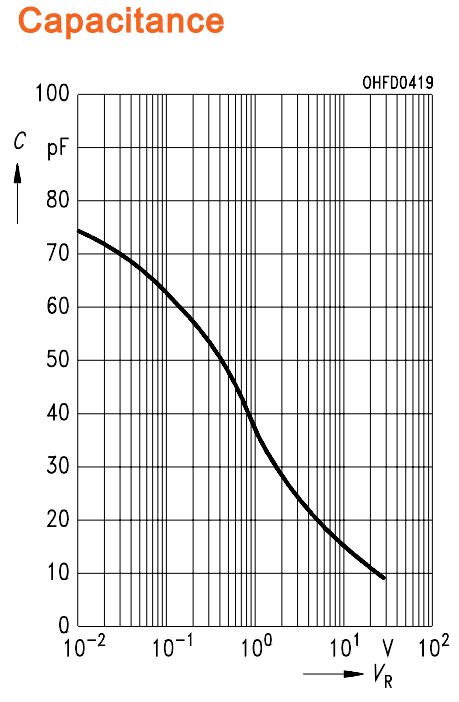
\includegraphics[width=6cm]{images/TD/SFH206_capa.png}
\end{figure}
	
	\item Que valent $\omega_T$ et $m_T$ pour $V_R = 0\operatorname{V}$ ? Pour $V_R = 30\operatorname{V}$ ?	
	\item Quelles formes ont les réponses en fréquence pour ces deux valeurs de tension de polarisation ?
	\item Parmi les deux réponses indicielles suivantes, laquelle est celle pour $V_R = 0\operatorname{V}$ ? Pour $V_R = 30\operatorname{V}$ ?
\begin{figure}[!h]
	\centering
	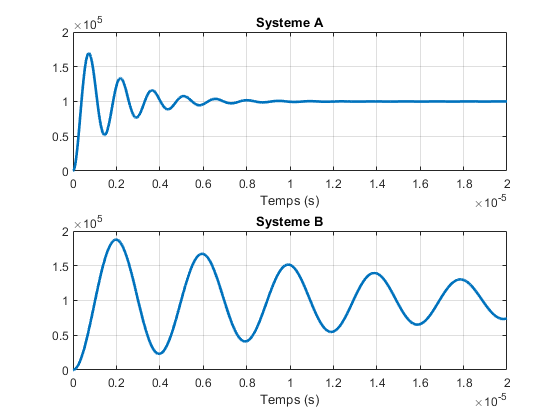
\includegraphics[width=10cm]{images/TD/step_sys.png}
\end{figure}
\end{enumerate}

